\chapter{Adjoint method}



\section{Automatic Differentiation}

%TODO: Togli questa prima parte, comincia direttamente con il come calcolare le derivate
%Automatic Differentiation (AD) is a family of techniques similar to but more general then backpropagation to efficiently and accurately evaluating derivatives of numeric functions expressed as computer programs. Backpropagation is a well known algorithm used in machine learning and artificial intelligence toolbox being the mainstay for training neural networks. Became popular with the work of Rumelhart in~\cite{Rumelhart:backpropagation_algo} it consists in learning the best set of weights for the network that minimize a certain objective function via an iterative procedure; to do so, for each weights update, a gradient in the weight space has to be computed. The aforementioned gradient is computed by the backpropagation of the sensitivity of the objective function at the output utilizing the chain rule to compute partial derivatives of the objective with respect to each weight. This algorithm is essentially equivalent to the derivative computation via reverse mode AD.

In general there exists different ways to compute derivatives using a computer program, these are:
\begin{description}
	\item[Manual Differentiation] In this case \emph{analytical} derivatives are computed by hand and then are plugged into standard optimization procedures such as gradient descend. Of course doing so is time consuming and prone to error;
	
	\item[Numerical Differentiation] In this case finite difference methods, as the ones reported in subsection~\vref{subsec:finite_difference_methods}, are used to approximate the derivatives \emph{values}. Easy to implement it has the disadvantage to be inaccurate due to round-off and truncation errors;

	\item[Symbolic Differentiation] This case addresses the weakness of both manual and numerical differentiation. \emph{Analytical} derivative expressions are automatically obtained by modern computer algebra systems such as Mathematica or SimPy [cita]. Unfortunately, often, the outcomes are plagued with the problem of ``expression swell'' which means that the resulting expressions are large, complex and cryptic;
	% TODO: Aggiungi li problema che algorithmic control-flow viene perso
	%TODO: cita il fatto dell'expression swell
	\item[Automatic Differentiation] This last case refers to a family of techniques that compute derivative \emph{values} (in contrast with symbolic differentiation) by using symbolic rules of differentiation (but keeping track of derivative values as opposed to the resulting
	expressions) through accumulation of values during code execution. The mix between symbolic and numerical differentiation gives to these methodologies an hybrid nature.
	%TODO: they also have the advantage of for and if working
	%TODO: There are two families
\end{description}

For the remaining of this section we will explain the details of Automatic Differentiation (AD), to do so we will look at its two (main) implementations:
\begin{itemize}
	\item Forward mode, also known as tangent linear mode;
	\item Reverse mode, also known as cotangent linear mode or \emph{adjoint} mode.
\end{itemize}
To showcase how each of the two modes works, we show how they are applied to a function $\tilde{f} \colon \R^2 \to \R^2$ defined as:
\begin{equation}
	\label{eqn:example_function_for_AD}
	\tilde{f}(x_1, x_2) = \begin{bmatrix}
					\tilde{f}_1(x_1, x_2)  &  \tilde{f}_2(x_1, x_2)
				  \end{bmatrix}
\end{equation}
with $\tilde{f}_1(x_1, x_2) = x_1 x_2 + \cos x_1$ and $\tilde{f}_2(x_1, x_2) = x_2^3 + \ln x_1 - x_2$.

Before entering into the detail we notice that every function $f \colon \R^n \to \R^m$ can be rewritten as a computational graph. A computational graph is a direct graph whose nodes correspond to operations and each operation can feed its output into other operations; once the graph is fed with some variables each node become automatically function of those variables. The usual operations considered as nodes are: binary arithmetic operations, the unary sign switch and transcendental functions such as exponential, logarithm and trigonometric functions.
Creating a computational graph for a function becomes easy by indicating with:
\begin{itemize}
	\item $v_{i-n}=x_i$, $i=1, \dots, n$ the input variables;
	\item $v_i$, $i=1, \dots, l$ the intermediate variable;
	\item $y_{m-i}=v_{l-i}$, $i=m-1, \dots, 0$ the output variables.
\end{itemize}
To better identify the relationship between the elementary operations which constitute a function it is helpful creating an \emph{evaluation trace}, also called Wenger list, of the function itself.
Left-hand side of table~\ref{tab:forward_AD_example} and figure~\ref{fig:example_of_computational_graph} contains respectively the evaluation trace and the computational graph for function $\tilde{f}$.

\begin{figure}
\centering
\begin{tikzpicture}
	[circle, inner sep=0pt, minimum size=10mm,
	operation/.style={draw},
	input/.style={draw=none},
	output/.style={draw=none}, -latex, auto, semithick]
	
	
	\node[operation] (v_minus_one) 				   								   {$v_{-1}$};
	\node[operation] (v_zero)	   [below=of v_minus_one, yshift=-20mm] 		   {$v_0$};
	\node[input]	 (x_one)	   [left=of v_minus_one] 						   {$x_1$};
	\node[input]	 (x_two)	   [left=of v_zero] 							   {$x_2$};
	
	\node[operation] (v_one)       [right=of v_minus_one, xshift=5mm, yshift=10mm] {$v_1$};
	\node[operation] (v_two)       [below=of v_one] 							   {$v_2$};
	\node[operation] (v_three)     [below=of v_two] 							   {$v_3$};
	\node[operation] (v_four)      [below=of v_three] 							   {$v_4$};
	
	\node[operation] (v_six)       [right=of v_four, xshift=5mm] 				   {$v_6$};
	
	\node[operation] (v_seven)     [right=of v_six, xshift=5mm, yshift=10mm] 	   {$v_7$};
	\node[operation] (v_five)      [above=of v_seven, yshift=20mm] 			   	   {$v_5$};
	\node[output]	 (f_one)	   [right=of v_five] 							   {$f_1(x_1,x_2)$};
	\node[output]	 (f_two)	   [right=of v_seven] 							   {$f_2(x_1,x_2)$};
	
	
	\draw [->] (x_one)		 to (v_minus_one);
	\draw [->] (x_two)		 to (v_zero);
	\draw [->] (v_minus_one) to (v_one);
	\draw [->] (v_minus_one) to (v_two);
	\draw [->] (v_minus_one) to (v_four);
	\draw [->] (v_zero) 	 to (v_two);
	\draw [->] (v_zero) 	 to (v_three);
	\draw [->] (v_zero) 	 to (v_seven);
	\draw [->] (v_one)		 to (v_five);
	\draw [->] (v_two)		 to (v_five);
	\draw [->] (v_three)	 to (v_six);
	\draw [->] (v_four)	 	 to (v_six);
	\draw [->] (v_six)		 to (v_seven);
	\draw [->] (v_five)		 to (f_one);
	\draw [->] (v_seven)	 to (f_two);
\end{tikzpicture}
\caption{Computational graph of function $\tilde{f}(x_1, x_2) = \Bigl[
		\tilde{f}_1(x_1, x_2) \,\, \tilde{f}_2(x_1, x_2) \Bigr]$. Definitions of intermediate variables $ v_{-1}, \dots, v_7$ can be found in table~\ref{tab:forward_AD_example} or table~\ref{tab:reverse_AD_example}}
\label{fig:example_of_computational_graph}
\end{figure}

Using the aforementioned representations we see that every function ultimately is a composition of elementary operations. This also means that its numerical derivatives can be computed by combining all the numerical derivatives of the constituent operations through the \emph{chain rule}: this, is the main idea of AD.

%TODO: 1) Talk about automatic label misconception
%Before going ahead we would like to draw reader's attention on the risk of ambiguity that the term ``automatic'' in  AD generate. One might label as AD every technique that allows to compute derivatives without computing them manually (e.g. Symbolic Differentiation), but in technical terms AD is used to indicate only those techniques that compute derivatives through accumulation of values during code execution to generate numerical numerical derivative evaluations rather than derivative expression.

%TODO: 2) Talk about that AD work also with regular code constructs
%We also emphasize the advantage of AD that can be applied to regular code with minimal change, allowing branching, loops and recursion unlike manual and symbolic differentiation which require to arrange the code under the syntactic and semantic constraint of the obtained formulas.


\subsection{Forward mode}
\label{subsec:forward_mode_AD}

In order to compute the derivative of the function $\tilde{f}$, reported in~\eqref{eqn:example_function_for_AD}, respect to $x_1$ we start by considering the evaluation trace on the left-hand side of table~\ref{tab:forward_AD_example} and we associate to each intermediate variable $ v_i$ the derivative:
\[
	v_i' = \frac{\partial v_i}{\partial x_1}
\]
Moving from top to bottom in the forward primal trace the corresponding tangent (derivative) trace, presented on the right-hand side of table~\ref{tab:forward_AD_example}, is generated by applying the chain rule to each encountered operation. After the primals $v_i$ are evaluated, also the corresponding tangents $v_i'$ are, again, from top to bottom; this gives us the desired derivatives in the final variables $v_5' = \frac{\partial y_1}{\partial x_1}$ and $v_7' = \frac{\partial y_2}{\partial x_1}$.
%One of the advantages using this implementation is that, in just one forward pass, we obtained all the derivatives respect $x_1$.
%TODO: Cite the fact the output is exact except for floating point appprox
%TODO Cite that derivatives are computed at the same time of the evauation of forward primal trace

\medskip
Forward mode can also be employed to evaluate the Jacobian of a generic function $f \colon \R^n \to \R^m$ at a point $\vec{x} = \vec{a}$ by performing $n$ distinct forward passes. By setting only one variable $x_i'=1$ and the others to zero we obtain:
\[
	y_j' = \frac{\partial y_j}{\partial x_i}\bigg|_{\vec{x}=\vec{a}} \qquad j=1,\dots,m.
\]
and reiterating for $i=1,\dots,n$, placing the resulting vectors side by side, we eventually obtain the Jacobian of $f$:
\[
\vec{J}_f =
\left.
\begin{bmatrix}
	\frac{\partial y_1}{\partial x_1} &  \dots  & \frac{\partial y_1}{\partial x_n}  \\
	\vdots							  & \ddots  & \vdots							 \\
	\frac{\partial y_m}{\partial x_n} &  \dots  & \frac{\partial y_m}{\partial x_n}
\end{bmatrix}
\right|_{\vec{x} = \vec{a}}
\]

Furthermore, by properly fine-tuning the values of the variables $x_1', \dots, x_n'$ is possible computing efficiently and in a matrix-free way Jacobian-vector products:
\[
\vec{J}_f \vec{r} =
\begin{bmatrix}
	\frac{\partial y_1}{\partial x_1} &  \dots  & \frac{\partial y_1}{\partial x_n}  \\
	\vdots							  & \ddots  & \vdots							 \\
	\frac{\partial y_m}{\partial x_1} &  \dots  & \frac{\partial y_m}{\partial x_n}
\end{bmatrix}
\begin{bmatrix}
	r_1		\\
	\vdots  \\
	r_n
\end{bmatrix}
\]
To accomplish this all that needs to be done is simply initializing $\vec{x}'=\big[x_1', \dots, x_n' \big]$ with $\vec{r}$; this result is particularly important in the evaluation of directional derivatives.
Before moving on, it is crucial to point out that forward mode AD:
\begin{itemize}
	\item for a function $f \colon \R \to \R^m$ allows to evaluate all its derivatives in just one forward pass, regardless of $m$;
	\item for a scalar field $f \colon \R^n \to \R$, the evaluation of its gradient $\nabla f = \Bigl[ \frac{\partial y}{\partial x_1}, \dots, \frac{\partial y}{\partial x_n} \Bigr]$ always require $n$ evaluations (since gradient is nothing more than a Jacobian of size $1 \times n$).
	%TODO: Add note of the factthat that it is not advantageous respect others methods
\end{itemize}
This means that the here explained implementation of AD is effective during the computation of derivative for cases $f \colon \R^n \to \R^m$ where $n \ll m$. For cases $n \gg m$ \emph{reverse mode} is more beneficial; we will discover why in the following subsection.

\begin{table}
\centering
	\begin{tabular}{cll}
		\toprule
		\multicolumn{3}{l}{\text{Forward Primal Trace}}  	 \\
		$v_{-1}$ &  $=x_1$ 				  & $=2$  			 \\
		$v_0$	 &  $=x_2$ 				  & $=3$  			 \\
		\midrule
		$v_1$	 &  $=\cos v_{-1}$  	  & $=\cos 2$      	 \\
		$v_2$	 &  $=v_{-1}  v_0$  	  & $=2 \cdot 3$  	 \\
		$v_3$	 &  $=v_0^3$  			  & $=3^3$	  	  	 \\
		$v_4$	 &  $=\ln v_{-1}$  	  	  & $=\ln 2$  	  	 \\
		$v_5$	 &  $=v_2 + v_1 \quad$    & $=6-0.416$   	 \\
		$v_6$	 &  $=v_3 + v_4$  		  & $=27+0.693$  	 \\
		$v_7$	 &  $=v_6 - v_0$  		  & $=27.693-3$  	 \\
		\midrule
		$y_1$	 &  $=v_5$				  & $=5.584$		 \\
		$y_2$	 &  $=v_7$				  & $=24.693$		 \\
		\bottomrule
	\end{tabular}
%	\begingroup\setlength{\fboxsep}{0pt}
%	\colorbox{lightgray}{
		\begin{tabular}{cll}
			\toprule
			\multicolumn{3}{l}{\text{Forward Tangent (Derivative) Mode}}  							 \\
			$v'_{-1}$ 		 &  $=x'_1$						  			& $=1$  					 \\
			$v'_0$	  		 &  $=x'_2$ 					  			& $=0$  					 \\
			\midrule
			$v_1'$	  		 &  $=-v_{-1}'\sin v_{-1}$  	  			& $= -1 \cdot \sin 2$      	 \\
			$v_2'$	  		 &  $=v_{-1}'  v_0 + v_{-1}  v_0' \quad$	& $=1 \cdot 3 + 2 \cdot 0$ 	 \\
			$v_3'$	  		 &  $=3  v_o^2  v_0'$  						& $=3 \cdot 2^2 \cdot 0$  	 \\
			$v_4'$	  		 &  $=v_{-1}' / v_{-1}$  			  		& $=1/2$	  	  	 		 \\
			$v_5'$	  		 &  $=v_2' + v_1'$  		  				& $=3 - 0.909$   	 		 \\
			$v_6'$	  		 &  $=v_3' + v_4'$  		  				& $=0+0.5$  	  			 \\
			$v_7'$	  		 &  $=v_6' - v_0'$  		  				& $=0.5 - 0$  				 \\
			\midrule
			$\mathbf{y'_1}$	 &  $\mathbf{=v_5'}$				  		& $\mathbf{=2.091}$			 \\
			$\mathbf{y'_2}$	 &  $\mathbf{=v_7'}$				  		& $\mathbf{=0.5}$			 \\
			\bottomrule
		\end{tabular}
%	} \endgroup
\caption{Forward mode AD example to evaluate the derivatives $\frac{\partial y_1}{\partial x_1}$ and $\frac{\partial y_2}{\partial x_1}$ of $\tilde{f}(x_1, x_2)$ at $[x_1, x_2] = [2,3]$. $x_1'$ and $x_2'$ are respectively set to $1$ and $0$ in order to derive only respect $x_1$. On the left is reported the forward evaluation trace, on the right the tangent one}
\label{tab:forward_AD_example}
\end{table}

%TODO: 1) Aggiungi colore alla tabella di dx
%TODO: 2) Aggiungi descrizione tabelle
%TODO: 3) Aggiungi frecce alle tabelle

\subsection{Reverse mode}
\label{subsec:reverse_mode_AD}

In this case, as opposed to forward mode AD, the derivatives are propagated back from a given output. A demonstration of how it works is presented in table~\ref{tab:reverse_AD_example} where we compute the sensitivities of output $y_1 = \tilde{f}_1(x_1, x_2)$ of $\tilde{f}$ respect the inputs $x_1$ and $x_2$. Different variables, called adjoints, are associated to each variable $v_i$ of the Forward Primal Trace and each of them is defined as:
\[
\overline{v}_i = \frac{\partial y_j}{\partial v_i}
\]
An adjoint variable is nothing more than the sensitivity of the output $y_j$ with respect to changes in $v_i$. It is important for the reader to note that, with this mode, the variable with respect to the derivatives are computed is not fixed as in forward mode AD.

Since typical usage of chain rule is forward derivatives propagation, reverse mode AD might appear confusing at first sight; to make it clearer we show how the chain rule can be used to back-propagating derivatives in order to compute the contribution $\overline{v}_0$ of the change in variable $v_0$ to the change in the output $y_1$. From figure~\ref{fig:example_of_computational_graph} can be seen that the only way variable $v_0$ can affect $y_1$ is through affecting $v_2$ and $v_3$, so its contribution to the change in $y_1$ can be computed using the chain rule as follow:
\begin{equation}
	\frac{\partial y_1}{\partial v_0} = \frac{\partial y_1}{\partial v_2} \frac{\partial v_2}{\partial v_0} + \frac{\partial y_1}{\partial v_3} \frac{\partial v_3}{\partial v_0}
\end{equation}
which can be rewritten in
\begin{equation}
	\begin{split}
		\frac{\partial y_1}{\partial v_0} & = \overline{v}_2 \frac{\partial v_2}{\partial v_0} + \overline{v}_3 \frac{\partial v_3}{\partial v_0}  \\[2ex]
										  & = \overline{v}_2 v_{-1} + 3 \overline{v}_3 v_0^2
	\end{split}
\end{equation}
where quantities $\overline{v}_2$ and $\overline{v}_3$ are known and derivatives $\frac{\partial v_2}{\partial v_0}$, $\frac{\partial v_3}{\partial v_0}$, can be easily computed by evaluating the result of symbolic differentiation of the elementary operations on the primals $v_i$.

\medskip
In light of the previous example, it is clear that, to compute derivatives, primals $v_i$ must be known along their dependencies within the computational graph. To do so two phases are required:
\begin{itemize}
	\item A \emph{forward step} where variables $v_i$ are populated and their dependencies recorded;
	\item A \emph{reverse step} where adjoints $\overline{v}_i$ are evaluated from outputs to inputs using values obtained in the first step.
\end{itemize}
We remark that once the backward pass is completed we get \emph{all} the sensitivities $\frac{\partial y_j}{\partial x_1}, \dots, \frac{\partial y_j}{\partial x_n}$ in one single pass; this means that for scalar fields $f \colon \R^n \to \R$ the computation of the gradient $\nabla f$ require only one application of reverse mode as opposed to the $n$ passes required in case of forward mode. Nevertheless, this advanatage comes at the cost of increased memory requirements which grows proportionally (in the worst case) to the number of operations in the evaluated function~\cite{Baydin:AD_survey}.

Generalizing the reasoning to functions $f \colon \R^n \to \R^m$, similarly to how it was done in previous section, we can conclude that reverse mode AD can also be used to evaluate Jacobians at a point; in particular, since each pass of reverse AD allows to compute one row of the Jacobian, its usage is advantageous when $m \ll n$ .
With regard to products between Jacobain and vector, reverse AD allows to compute efficiently vector-Jacobian products of type:
\begin{equation}
	\vec{r}^T \vec{J}_f =
	\begin{bmatrix}
		r_1 	& \dots  & r_m
	\end{bmatrix}
	\begin{bmatrix}
		\frac{\partial y_1}{\partial x_1} &  \dots  & \frac{\partial y_1}{\partial x_n}  \\
		\vdots							  & \ddots  & \vdots							 \\
		\frac{\partial y_m}{\partial x_1} &  \dots  & \frac{\partial y_m}{\partial x_n}
	\end{bmatrix}
\end{equation}
by initializing $\vec{\overline{y}}=\big[\overline{y}_1, \dots, \overline{y}_m \big]$ with $\vec{r}$.

\begin{table}
	\centering
	\begin{tabular}{cll}
		\toprule
		\multicolumn{3}{l}{\text{Forward Primal Trace}}  	 \\
		$v_{-1}$ &  $=x_1$ 				  & $=2$  			 \\
		$v_0$	 &  $=x_2$ 				  & $=3$  			 \\
		\midrule
		$v_1$	 &  $=\cos v_{-1}$  	  & $=\cos 2$      	 \\
		$v_2$	 &  $=v_{-1}  v_0$  	  & $=2 \cdot 3$  	 \\
		$v_3$	 &  $=v_0^3$  			  & $=3^3$	  	  	 \\
		$v_4$	 &  $=\ln v_{-1}$  	  	  & $=\ln 2$  	  	 \\
		$v_5$	 &  $=v_2 + v_1 \quad$    & $=6-0.416$   	 \\
		$v_6$	 &  $=v_3 + v_4$  		  & $=27+0.693$  	 \\
		$v_7$	 &  $=v_6 - v_0$  		  & $=27.693-3$  	 \\
		\midrule
		$y_1$	 &  $=v_5$				  & $=5.584$		 \\
		$y_2$	 &  $=v_7$				  & $=24.693$		 \\
		\bottomrule
	\end{tabular}
	%	\begingroup\setlength{\fboxsep}{0pt}
	%	\colorbox{lightgray}{
	\begin{tabular}{clll}
		\toprule
		\multicolumn{4}{l}{\text{Forward Tangent (Derivative) Mode}}  							 \\
		$\mathbf{\overline{x}_1}$  &  $\mathbf{ =\frac{\partial y_1}{\partial v_{-1}} \frac{\partial v_{-1}}{\partial x_1} }$  & $\mathbf{=\overline{v}_{-1} \cdot 1 }$  &  $=2.091$  \\
		$\mathbf{\overline{x}_2}$  &  $\mathbf{ =\frac{\partial y_1}{\partial v_0} \frac{\partial v_0}{\partial x_2}}$  	   &  $\mathbf{ =\overline{v}_0 \cdot 1 }$   &  $=2$		  \\
		
		\midrule
		$\overline{v}_{-1}$  &  $=\frac{\partial y_1}{\partial v_1} \frac{\partial v_1}{\partial v_{-1}} + \frac{\partial y_1}{\partial v_2} \frac{\partial v_2}{\partial v_{-1}} + \frac{\partial y_1}{\partial v_4} \frac{\partial v_4}{\partial v_{-1}}$  &  $=-\overline{v}_1 \sin (v_{-1}) + \overline{v}_2 v_0 + \overline{v}_4/v_{-1}$  &  $=2.091$  \\
		$\overline{v}_0$	 &  $=\frac{\partial y_1}{\partial v_2} \frac{\partial v_2}{\partial v_0} + \frac{\partial y_1}{\partial v_3} \frac{\partial v_3}{\partial v_0}$  & $=\overline{v}_2 v_{-1} + 3 \overline{v}_3 v_0^2$  &  $=2$  \\
		$\overline{v}_1$	 &  $=\frac{\partial y_1}{\partial v_5} \frac{\partial v_5}{\partial v_1}$  &  $=\overline{v}_5 \cdot 1$  &  $=1$  \\
		$\overline{v}_2$	 &  $=\frac{\partial y_1}{\partial v_5} \frac{\partial v_5}{\partial v_2}$  &  $=\overline{v}_5 \cdot 1$  &  $=1$  \\
		$\overline{v}_3$	 &  $=\frac{\partial y_1}{\partial v_6} \frac{\partial v_6}{\partial v_3}$  &  $=\overline{v}_6 \cdot 1$  &  $=0$  \\
		$\overline{v}_4$	 &  $=\frac{\partial y_1}{\partial v_6} \frac{\partial v_6}{\partial v_4}$  &  $=\overline{v}_6 \cdot 1$  &  $=0$  \\
		$\overline{v}_6$	 &  $=\frac{\partial y_1}{\partial v_7} \frac{\partial v_7}{\partial v_6}$  &  $=\overline{v}_7 \cdot 1$  &  $=0$  \\
		
		\midrule
		$\overline{v}_5$  &  $=\overline{y}_1$	&  &  $=1$	\\
		$\overline{v}_7$  &  $=\overline{y}_2$  &  &  $=0$	\\
		\bottomrule
	\end{tabular}
	%	} \endgroup
	\caption {Reverse mode AD example with $[y_1, y_2] = \tilde{f}(x_1, x_2)$ evaluated at $[x_1, x_2] = [2,3]$. First, primal trace is evaluated (table above) and then adjoint variables are computed, from the  bottom up, in a second phase (table below). The initialization $\overline{v}_5 = \frac{\partial y_1}{\partial v_5} = \frac{\partial y_1}{\partial y_1} = \overline{y}_1 = 1$ and $\overline{v}_7 = \frac{\partial y_1}{\partial v_7} = \frac{\partial y_1}{\partial y_2} = \overline{y}_2 = 0$ is such that it allows the sensitivities to be calculated with respect the fist output}
%	\caption{Reverse mode AD example to evaluate the derivatives $\frac{\partial y_1}{\partial x_1}$ and $\frac{\partial y_1}{\partial x_2}$ of $\tilde{f}(x_1, x_2)$ at $[x_1, x_2] = [2,3]$. $y_1'$ and $y_2'$ are respectively set to $1$ and $0$ in order to obtain the sensitivities respect $y_1$. Above is reported the forward evaluation trace, below the adjoint one}
	\label{tab:reverse_AD_example}
\end{table}


% which gives the contribution $\overline{v}_i$ of the change in each variable $v_i$ to the change in the output $y_j$


%TODO: Aumenta l'altezza delle righe della tabella con \\[2ex] come spiegato nell'Arte a pag. 129
%TODO: Valuta la notazione $\vec{\overline{y}}$ che è un po' ambigua nel caso in cui cambi output da differenziare
%TODO: Cita più spesso AD survey 


\section{Application to design optimization}
\label{sec:application_to_design_opt}


\subsection{Introduction}

Design optimization is the process of finding the best design parameters $\vec{l} = [l_1, \dots, l_N]$ that satisfy project requirements~\cite{Matlab:design_opt}. Requirements and objectives, which are usually multiple and conflicting, are typically expressed in the form of a scalar function $J(\vec{u},\vec{l}) \colon \R^M\times\R^N \to \R$ named \emph{cost} or \emph{objective function}. $J$ depends on the design parameters $\vec{l} \in \R^N$ and the state $\vec{u} \in \R^M$ of the problem at hand; $\vec{u}$ is generally found as solution of a system of linear equations $\vec{Au} = \vec{b}$, which arise from the imposition of the constraints of the problem, where $\vec{A} \in \R^{M \times M}$ and $\vec{b} \in \R^M$ depends on some way on $\vec{l}$. In figure~\ref{fig:design_opt_scheme} can be found a scheme of this process.

This type of process is of interest since it is encountered in the most diverse fields, from computer science, where for example the proper weights of a neural network has to be found in order to minimize the error between its predicted and the desired output respect a given set of inputs, to mechanical engineering where one may want to modify the shape of an heat sink to maximize the amount of the heat transferred to the environment.

\begin{figure}
	\centering
	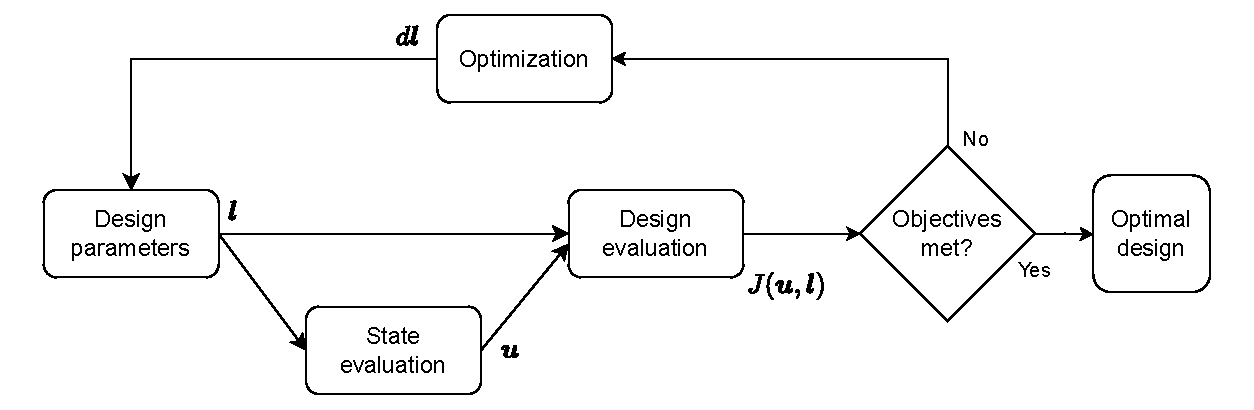
\includegraphics[width=\textwidth]{img/design_opt_scheme.pdf}
	\caption{Scheme of a design optimization process. From an initial design defined by a set of parameters $\vec{l}$ the associated state $\vec{u}$ is derived. The state in conjunction with the parameters are then used to evaluate the design through a function $J$. If the objectives are met the design is kept otherwise the whole procedure is repeated with a new set of parameters obtained by modifying the previous ones by a quantity $d\vec{l}$} 
	\label{fig:design_opt_scheme}
\end{figure}

To find the best parameters for a given project a variety of iterative approaches can be pursued:
\begin{description}
	\item[Manual approach] where each parameter $l_1, \dots, l_N$ is adjusted one at a time. Unfortunately doing so tends to leads to suboptimal results;
	\item[Brute-force approach] where all possible combinations of design parameters are evaluated. However, this is time-expensive and for large-scale projects, where parameters can be hundreds, thousands, or even more, optimal parameters may not be found in reasonable time-frames;
	\item[Gradient approach] where the gradient $\frac{dJ}{d\vec{l}}$ permits both to update all the parameters $l_1, \dots, l_N$ at the same time and to disregard most of the parameter values that are sub-optimal by considering only those suggested by its direction.
\end{description}
For the effectiveness of the last mentioned approach, is crucial to ensure an efficient computation of the gradient $\frac{dJ}{d\vec{l}}$ which must require as few steps as possible and be efficient even for problems involving huge number of design parameters. To meet these requirements Automatic Differentiation (AD) in its reverse-mode declination is necessary.
%TODO: adjust the end of the "paragraph"

\bigskip
Given its advantages in design optimization we have learned that using the gradient is a good course of action. To directly evaluate $\frac{dJ}{d\vec{l}}$, in case of a particular set of design parameters defined by $\vec{l}$ at a given state $\vec{u}$, we would compute:
\begin{equation}
	\label{eqn:generic_gradient_design_opt}
	\frac{dJ}{d\vec{l}}^T = \frac{\partial J}{\partial \vec{u}}^T \frac{d\vec{u}}{d\vec{l}} + \frac{\partial J}{\partial \vec{l}}^T
\end{equation}
%TODO: Valuta di precisare la notazione da qualce parte invece di metterla in mezzo al documento
where notations $\frac{d}{dx}$ and $\frac{\partial}{\partial x}$ indicate the total and the partial derivatives respect the variable $x$ respectively.
Of the required elements $\frac{\partial J}{\partial \vec{u}}$ and $\frac{\partial J}{\partial \vec{l}}$ can be efficiently obtained by means of reverse-mode AD, as explained in subsection~\vref{subsec:reverse_mode_AD}, since $J$ is known analytically. The matrix $\frac{d\vec{u}}{d\vec{l}}$, on the other hand, require more careful considerations.

Differentiating the problem constraints $\vec{Au} = \vec{b}$ respect the parameters $\vec{l}$ gives:
\begin{equation}
	\frac{d\vec{A}}{d\vec{l}} \vec{u} + \vec{A} \frac{d\vec{u}}{d\vec{l}} = \frac{d\vec{b}}{d\vec{l}}
\end{equation}
which allows to obtain the sought term $\frac{d\vec{u}}{d\vec{l}}$ as:
\begin{equation}
	\label{eqn:state_sensitivity_respect_single_param}
	\frac{d\vec{u}}{d\vec{l}} = \vec{A}^{-1} \left( \frac{d\vec{b}}{d\vec{l}} - \frac{d\vec{A}}{d\vec{l}}\vec{u} \right)
\end{equation}
We notice that $\frac{d\vec{u}}{d\vec{l}}$ is a matrix of size $M \times N$ whose $j$-th column represent the sensitivity of the state $\vec{u}$ respect parameter $l_j$. In practice it is populated column-wise by solving equation~\eqref{eqn:state_sensitivity_respect_single_param} $N$ times considering the vector $\vec{l}$ as the scalar $l_j$: this gives its $j$-th column. In this process $\frac{d\vec{b}}{d\vec{l}}$ and $\frac{d\vec{A}}{d\vec{l}}$ terms can be simply obtained using AD, if known analytically, and once $\frac{d\vec{u}}{d\vec{l}}$ is computed it can be substituted in equation~\eqref{eqn:generic_gradient_design_opt} to obtain the gradient which symbolically reads as:
\begin{equation}
	\label{eqn:generic_gradient_design_opt_naive}
	\frac{dJ}{d\vec{l}} = \frac{\partial J}{\partial \vec{u}}^T \left[ \vec{A}^{-1} \left( \frac{d\vec{b}}{d\vec{l}} - \frac{d\vec{A}}{d\vec{l}}\vec{u} \right) \right]  + \frac{\partial J}{\partial \vec{l}}^T
\end{equation}

However the computational costs of this naive procedure scales linearly with the number of the design parameters $N$ since $N$ inversions of matrix $\vec{A}$ are required for a single gradient computation. We finally remark that each of these inversions has the same computational cost of solving $\vec{A} \vec{u}= \vec{b}$ for $\vec{u}$ and if the solution represent the output of a particularly time consuming computation, as a a CFD simulation is an example of, this is particularly penalizing. A more efficient gradient computation is therefore required.

To do so we can employ the \emph{adjoint method} which simply consist of a smarter bracketing of the equation which gives the gradient. In fact is possible to rewrite~\eqref{eqn:generic_gradient_design_opt_naive} as:
\begin{equation}
	\begin{aligned}
		\frac{dJ}{d\vec{l}} & = \left[ \frac{\partial J}{\partial \vec{u}}^T \vec{A}^{-1} \right] \left( \frac{d\vec{b}}{d\vec{l}} - \frac{d\vec{A}}{d\vec{l}}\vec{u} \right) + \frac{\partial J}{\partial \vec{l}}^T  \\
							& = \vec{\lambda}^T \left( \frac{d\vec{b}}{d\vec{l}} - \frac{d\vec{A}}{d\vec{l}}\vec{u} \right) + \frac{\partial J}{\partial \vec{l}}^T
	\end{aligned}
\end{equation}
where the vector $\vec{\lambda} \in \R^L$, whose elements are called \emph{adjoint variables}, can be found by solving:
\begin{equation}
	\label{eqn:generic_adjoint_system_design_opt}
	\vec{A}^T \vec{\lambda} = \frac{\partial J}{\partial \vec{u}}
\end{equation}

By doing so is possible to solve the system in equation~\eqref{eqn:generic_adjoint_system_design_opt}, which is called \emph{adjoint problem}, only \emph{once} independently on the number $N$ of design parameters for each gradient computation: this significantly reduces the computational burden of the whole optimization process. Note that the adjoint problem has the same size as the problem defined by the constraints $\vec{A} \vec{u} = \vec{b}$ and the computational cost for their solution is the same.

\bigskip
At this point it is worth noting that the adjoint method explained above is just a particular application of reverse mode automatic differentiation. To make the connections between the two methods clearer we note that the first computation of the  objective function's gradient, presented in equation~\eqref{eqn:generic_gradient_design_opt}, contains the following vector-Jacobian product:
\begin{equation}
	\label{eqn:vJp_design_opt}
	\frac{\partial J}{\partial \vec{u}}^T \frac{d\vec{u}}{d\vec{l}}
\end{equation}
where $\frac{\partial J}{\partial \vec{u}}^T \in \R^M$ is the vector that multiply $\frac{d\vec{u}}{d\vec{l}} \in \R^{M \times N}$, the Jacobian of the state $\vec{u}$ respect the design parameters $\vec{l}$.
From subsection~\vref{subsec:reverse_mode_AD} we known that AD allows to compute the resulting vector without explicitly computing the Jacobian $\frac{d\vec{u}}{d\vec{l}}$. But this is precisely what the adjoint method does through equations~(\ref{eqn:generic_gradient_design_opt} -~\ref{eqn:generic_adjoint_system_design_opt}) by first applying the chain rule to the leftmost term in the gradient formula and then parenthesizing the result in order to make the number of inversions of the matrix $\vec{A}$ independent on the number of parameters.
The result of the whole process is then summarized by:
\begin{equation}
	\label{eqn:resulting_term_adjoint_method}
	\vec{\lambda}^T \left( \frac{d\vec{b}}{d\vec{l}} - \frac{d\vec{A}}{d\vec{l}}\vec{u} \right)
\end{equation}
where $\vec{\lambda}$ solves equation~\eqref{eqn:generic_adjoint_system_design_opt} and the Jacobian $\frac{d\vec{u}}{d\vec{l}}$ is no more present. Furthermore the two-steps process of the reveres mode AD for the gradient computation is still there even in the adjoint method:
\begin{itemize}
	\item the forward pass, used for the computation of variables $v_i$ in table~\vref{tab:reverse_AD_example}, now is the single solution of the system $\vec{A}\vec{u}=\vec{b}$ in order to find the state $\vec{u}$ used in term~\eqref{eqn:resulting_term_adjoint_method};
	\item the reverse pass, done in order to obtain the adjoint variables $\overline{v}_i$ in table~\ref{tab:reverse_AD_example}, is now equivalent to the solution of $\vec{A}^T \vec{\lambda} = \frac{\partial J}{\partial \vec{u}}$ (we would like to reiterate again that reverse and forward pass has the \emph{same} computational complexity). 
\end{itemize}
%TODO: Ingrandisci un po' le parentesi quadre


\section{Application to RBF-FD}

%As we have seen in section~\vref{sec:RBF-FD} RBF-FD solver is simply a numerical method employed in the solution of Partial Differential Equations (PDEs). Computational Fluid Dynamics (CFD) is one of the main areas of its application where the solver is applied to PDEs involving fluid flows and heat transfers. In all these cases design optimization problems arises almost naturally: regarding heat transfers we have already mentioned the heath sink case, as to fluid flows a typical example is to find the best shape for the wings of an aircraft in order to maximize its lift and/or minimize its drag.
%
%In these cases is possible to modify the geometry of the problems, e.g. the shape of the heat sink case or the wing's shape, by modifying some design parameters $\vec{l} \in \R^L$.
%Their perturbations therefore modify the physical domain $\Omega\cup\partial\Omega$ on which the RBF-FD method is applied.
%This means that the whole discretization process of the PDE's problem is affected which in turn affect the state of the problem which is defined as the output $\vec{u}_I$ of the RBF-FD procedure and is needed to evaluate the geometry through a cost function $J(\vec{u}_I, \vec{l})$ (e.g. the amount of lift/drag), The rest of this subsection will be devoted explaining how the adjoint method is employed for optimization in case of 1D or 3D problems.
%
%For both 1D ($\Omega\cup\partial\Omega \subseteq \R$) and 3D ($\Omega\cup\partial\Omega \subseteq \R^3$) cases the following optimization problem hast to be solved:
%\begin{equation}
%	\min_{\vec{l}}
%\end{equation}

%In these design optimization problems the advantages of Meshless Methods (MMs) respect the traditional FEM adn FVM methods are even more important. Typical solvers require the creation of a mesh which leads 

%For the specific case of RBF-FD methods the design optimization problem come down to 

\subsection{1D}
\label{subsec:adjoint_method_RBF-FD_1D}

In this case we consider a general cost function $J \colon \R^{N_I \times L} \to \R$. Thanks to this generality its sensitivities respect the design parameters are given by the same exact formula used in general design optimization problems:
\begin{equation}
	\label{eqn:}
	\frac{dJ}{d\vec{l}}^T = \frac{\partial J}{\partial \vec{u}_I}^T \frac{d\vec{u}_I}{d\vec{l}} + \frac{\partial J}{\partial \vec{l}}^T
\end{equation}
Once more, what is now lacking is the term $\frac{d\vec{u}_I}{d\vec{l}}$. The sensitivities of the state respect the parameters can be computed by differentiating equation ()
% C_I * u_I = f - C_B * u_B da aggiungere nell'intro della section
which gives
\begin{equation}
	\label{eqn:gradient_1st_step_1D_RBF-FD}
	\frac{d\vec{C}_I}{d\vec{l}} \vec{u}_I + \vec{C}_I \frac{d\vec{u}_I}{d\vec{l}} + \frac{d\vec{C}_B}{d\vec{l}} \vec{u}_B + \vec{C}_B \frac{d\vec{u}_B}{d\vec{l}} =
	\frac{d\vec{f}}{d\vec{l}}
\end{equation} 
Before proceeding a note on the matrix $\frac{d\vec{u}_B}{d\vec{l}}$ could be useful since one might think that it should not be present since values in $\vec{u}_B$ are fixed from boundary conditions of the boundary value problem~\vref{eqn:boundary_value_problem} (i.e. they are not dependent on the design parameters). The previous statements holds true only for Dirichlet BCs, but not in general since in case of Neumann and Robin BCs the values of $\vec{u}_B$ depends also on their normal derivatives respect the surface $\partial\Omega$ whose shape depends on $\vec{l}$. This simply means that only the rows of $\frac{d\vec{u}_B}{d\vec{l}}$ associated to Dirichlet points will make up of zeros elements.

Once $\frac{d\vec{u}_I}{d\vec{l}}$ is isolated from the previous equation it can be plugged in~\eqref{eqn:gradient_1st_step_1D_RBF-FD} which in turns become:
\begin{equation}
\begin{aligned}
	\frac{dJ}{d\vec{l}}^T & = \frac{\partial J}{\partial \vec{u}_I}^T \biggl[ \vec{C}_I^{-1} \biggl( \frac{d\vec{f}}{d\vec{l}} - \frac{d\vec{C}_I}{d\vec{l}} \vec{u}_I - \frac{d\vec{C}_B}{d\vec{l}} \vec{u}_B - \vec{C}_B \frac{d\vec{u}_B}{d\vec{l}} \biggr) \biggr] + \frac{\partial J}{\partial \vec{l}}^T  \\
						  & = \frac{\partial J}{\partial \vec{u}_I}^T \biggl[ \vec{C}_I^{-1} \biggl( \frac{d\vec{f}}{d\vec{l}} - \frac{d\vec{C}}{d\vec{l}} \vec{u} - \vec{C}_B \frac{d\vec{u}_B}{d\vec{l}} \biggr) \biggr] + \frac{\partial J}{\partial \vec{l}}^T
\end{aligned}
\end{equation}
where $\frac{d\vec{C}}{d\vec{l}} \in \R^{N_I \times N}$ is the matrix resulting from the concatenation of the rows of $\frac{d\vec{C}_I}{d\vec{l}} \in \R^{N_I \times N_I}$ and $\frac{d\vec{C}_B}{d\vec{l}} \in \R^{N_B \times N_B}$, and $\vec{u} \in \R^{N}$ is the vector given by the concatenation of the elements of $\vec{u}_I \in \R^{N_I}$ and $\vec{u}_B \in \R^{N_B}$.
Now the adjoint method can be employed in order to avoid performing the inversion of matrix $\vec{C}_I$ once for each parameter in $\vec{l}$, yielding:
\begin{equation}
	\frac{dJ}{d\vec{l}}^T =  \vec{\lambda}_1^T \biggl( \frac{d\vec{f}}{d\vec{l}} - \frac{d\vec{C}}{d\vec{l}} \vec{u} - \vec{C}_B \frac{d\vec{u}_B}{d\vec{l}} \biggr) + \frac{\partial J}{\partial \vec{l}}^T  \\
\end{equation}
where $\vec{\lambda}_1$ is found by solving \emph{once}:
\begin{equation}
	\vec{C}_I^T \vec{\lambda}_1 = \frac{\partial J}{\partial \vec{u}_I}
\end{equation}
The unknown terms involving derivatives computation on the right-hand side can be computed easily through AD except for $\frac{d\vec{C}}{d\vec{l}} \vec{u}$. This terms deserves more attentions since requires the differentiation of the global matrix $\vec{C}$ which is obtained by solving $N_I$ local systems, each associated with a different stencil $\mathcal{X}_i$.

\smallskip
%Taking a moment to consider the matrix $\frac{d\vec{C}}{d\vec{l}} \vec{u} \in \R^{N \times L}$ we can note that is obtained from a product between a rank-3 tensor 
In order to examine it more closely we can define a matrix $\vec{Q} \in \R^{N_I \times L}$ as follows:
\begin{equation}
	\vec{Q} = \frac{d\vec{C}}{d\vec{l}} \vec{u}
\end{equation}
whose elements $q_{i,j}$ are given by:
\begin{equation}
	\label{eqn:Q_elements}
	q_{i,j} = \frac{d\vec{C}_{[i,:]}}{dl_j} \vec{u}
\end{equation}
The notation $\vec{C}_{[i,:]}$ is used to indicate the $i$-th row of the matrix $\vec{C}$.
To obtain $\frac{d\vec{C}}{d\vec{l}} \vec{u}$ is thus sufficient to compute each element of $\vec{Q}$ through equation~\eqref{eqn:Q_elements}. However, before doing so, it is worth rewriting the equation for $q_{i,j}$ more explicitly.

Recall that elements that make up the $i$-th row of $\vec{C}$ are found by solving the local system~\eqref{eqn:row_of_C_system}:
\begin{equation}
	\vec{M_{BC}}^T
	\begin{bmatrix}
		\vec{c}_I(\vec{x}_i)  \\
		\vec{c}_B(\vec{x}_i)  \\
		\vec{c}_p(\vec{x}_i)
	\end{bmatrix} = 
	\begin{bmatrix}
		\mathcal{L} \vec{\Phi}(\vec{x}_i, \mathcal{X}_{i,I})  \\
		\mathcal{L} \vec{p}(\vec{x}_i)
	\end{bmatrix}
\end{equation}
in case of RBF-FD method, or the local system~\eqref{eqn:row_of_C_system_in_RBF-HFD}:
\begin{equation}
	\label{eqn:adjoint_method_row_of_C_system_in_RBF-HFD}
	\vec{M_{BC}}^T
	\begin{bmatrix}
		\vec{c}_I(\vec{x}_i)  \\
		\vec{c}_B(\vec{x}_i)  \\
		\vec{c}_p(\vec{x}_i)
	\end{bmatrix} = 
	\begin{bmatrix}
		\mathcal{L}_1 \vec{\Phi}(\vec{x}_i, \mathcal{X}_{i,I})  			  \\
		\mathcal{L}_1 \mathcal{B}_2 \vec{\Phi}(\vec{x}_i, \mathcal{X}_{i,B})  \\
		\mathcal{L} \vec{p}(\vec{x}_i)
	\end{bmatrix}
\end{equation}
in case of RBF-HFD method. The key aspect that both cases share is that the aforementioned equations arises from the information contained in a single stencil $\mathcal{X}_i$ and, as explained in subsection~\vref{subsec:RBF-FD_formulation}, only the first $m$ elements of $\vec{c}(\vec{x}_i) = \bigl[ \vec{c}_I(\vec{x}_i), \vec{c}_B(\vec{x}_i), \vec{c}_p(\vec{x}_i) \bigr]$ form the $i$-th row of $\vec{C}$. 
Furthermore, since $m \ll N$, row $\vec{C}_{[i,:]}$ is sparse; which in turns implies that not all the elements of $\vec{u}$ are involved in the computation of $q_{i,j}$.

By letting $\vec{\tilde{u}}_i \in \R^m$ the vector composed by the components of $\vec{u}$ associated to the non zero elements of $\vec{C}_{[i,:]}$, we can rewrite the elements of $\vec{Q}$ reported in~\eqref{eqn:Q_elements} as:
\begin{equation}
	\label{eqn:Q_elements_rewritten}
	q_{i,j} =
	\frac{\vec{c}(\vec{x}_i)^T}{dl_j}
	\begin{bmatrix}
		\vec{\tilde{u}}_i  \\
		\vec{0}
	\end{bmatrix}
\end{equation}
where the zero-vector concatenated to $\vec{\tilde{u}}_i$ has the same length of $\vec{c}_p(\vec{x}_i)$.
If we now differentiate equation~\eqref{eqn:adjoint_method_row_of_C_system_in_RBF-HFD} respect the $j$-th design parameter, we obtain:
\begin{equation}
	\frac{d \vec{M_{BC}}^T}{d l_j} \vec{c}(\vec{x}_i) + \vec{M_{BC}}^T \frac{d \vec{c}(\vec{x}_i)}{d l_j} = \frac{d \vec{h}}{d l_j}
\end{equation}
where the vector $\vec{h} \in \R^{m+M}$ is used as a shorthand for the vector present on the left-hand side of equation~\eqref{eqn:adjoint_method_row_of_C_system_in_RBF-HFD}. Now from the last equation we can isolate:
\begin{equation}
	\frac{d \vec{c}(\vec{x}_i)^T}{dl_j} = \left( \frac{d \vec{h}}{d l_j} - \frac{d \vec{M_{BC}}^T}{d l_j} \vec{c}(\vec{x}_i) \right)^T \vec{M_{BC}}^{-1}
\end{equation}
which once plugged in~\eqref{eqn:Q_elements_rewritten} allows to rewrite $q_{i,j}$ as:
\begin{equation}
	\label{eqn:Q_elems_before_adjoint}
	q_{i,j} =
	\left[ \left( \frac{d \vec{h}}{d l_j} - \frac{d \vec{M_{BC}}^T}{d l_j} \vec{c}(\vec{x}_i) \right)^T \vec{M_{BC}}^{-1} \right]
	\begin{bmatrix}
		\vec{\tilde{u}}_i  \\
		\vec{0}
	\end{bmatrix}
\end{equation}
But now we can clearly see that in order to populate the matrix $\vec{Q}$ we should invert $N_IL$ matrices $\vec{M_{BC}}$ of size $(m+M) \times (m+M)$ since we need to compute $\frac{d \vec{c}(\vec{x}_i)^T}{dl_j}$. These matrices are smaller than $\vec{C}_I$, but in any case their inversion is still problematic since usually both the number of parameters and the number of nodes within the physical domain are huge. The problem, here, is very similar to the one related to design optimization in section~\vref{sec:application_to_design_opt} where there was a linear relationship between the number of matrix inversions and the number of design parameters: consequently, even here, to improve the situation it is possible to rely on the adjoint method again. Modifying the parentheses of equation~\eqref{eqn:Q_elems_before_adjoint} it is possible to write:
\begin{equation}
	\begin{aligned}
		q_{i,j} & =
		\left( \frac{d \vec{h}}{d l_j} - \frac{d \vec{M_{BC}}^T}{d l_j} \vec{c}(\vec{x}_i) \right)^T
		\left(
		\vec{M_{BC}}^{-1}
		\begin{bmatrix}
			\vec{\tilde{u}}_i  \\
			\vec{0}
		\end{bmatrix}
		\right)  \\
				& =
		\left( \frac{d \vec{h}}{d l_j} - \frac{d \vec{M_{BC}}^T}{d l_j} \vec{c}(\vec{x}_i) \right)^T
		\vec{\lambda}_{2,i}
	\end{aligned}
\end{equation}
where the adjoint vector $\vec{\lambda}_{2,i} \in \R^{m+M}$ is found as solution of:
\begin{equation}
	\label{eqn:second_adjoint_in_RBF-HFD}
	\vec{M_{BC}} \vec{\lambda}_{2,i} =
	\begin{bmatrix}
		\vec{\tilde{u}}_i  \\
		\vec{0}
	\end{bmatrix}
\end{equation}
and has to be computed once for each row of $Q$ (or equivalently $\frac{d\vec{C}}{d\vec{l}} \vec{u}$). The crucial point is that this second adjoint implementation allows to make the computational cost to obtain $\frac{d\vec{C}}{d\vec{l}} \vec{u}$ independent of the number of design parameter $L$: the number of systems~\eqref{eqn:second_adjoint_in_RBF-HFD} that has to be solved, whose cost is similar to the inversion of $\vec{M_{BC}}$, is now always $N_I$.

\smallskip
In light of what we have been observed we are now able to compute the whole gradient $\frac{dJ}{d\vec{l}}^T$ with a computation effort analogous to two RBF-HFD:
\begin{enumerate}
	\item a first vanilla application of RBF-HFD is required in order to compute the terms $\vec{u}$, $\vec{C}_I$ and $\vec{C}_B$;
	\item then, a comparable cost is required for the application of the presented adjoint method as shown in table~\ref{tab:RBF-FD_and_adjoint_comparison}.
\end{enumerate}

\begin{table}
	\caption{Systems that demands the computation of a solution during the application of RBF-FD and the adjoint method explained in section~\ref{subsec:adjoint_method_RBF-FD_1D}. Those of dimension $m+M$ are solved once for each stencil in the physical domain}
	\label{tab:RBF-FD_and_adjoint_comparison}
	\centering
	\begin{tabular}{ccc}
		\toprule
		Method										&  Solved systems															& System dimension				\\
		\midrule
		\multirow{2}*{RBF-FD}						& $\vec{C}_I \vec{u}_I = f - \vec{C}_B \vec{u}_B$ 							& $N_I$							\\[1.5ex]
													& $\vec{M_{BC}}^T \vec{c}(\vec{x}_i) = \vec{h}$ for $i=1,\dots,N_I$								& $m+M$							\\[2ex]
		\multirow{2}*{Adjoint}						& $\vec{C}_I^T \vec{\lambda}_1 = \frac{\partial J}{\partial \vec{u}_I}$		& $N_I$							\\[1.5ex]
													& $\vec{M_{BC}} \vec{\lambda}_{2,i} =
													\begin{bmatrix}
														\vec{\tilde{u}}_i  \\
														\vec{0}
													\end{bmatrix}$ for $i=1,\dots,N_I$											& $m+M$						\\[1.5ex]
		\bottomrule
	\end{tabular}
\end{table}


%thus yields only $m$ elements, where $m$ is the number of nodes within the stencil. This means that $\vec{C}_{[i,:]}$ row is composed by just $m \ll N$ non-zero elements and thus not all the components of $\vec{u}$ are involved in the computation of $q_{i,j}$.
%By letting $\vec{\tilde{c}}_i$ represent the vector formed by the non-zero elements of $\vec{C}_{[i,:]}$ padded with a number of zero elements in order to and $\vec{\tilde{u}}_i$ the vector composed by the elements of $\vec{u}$ associated to $\vec{\tilde{c}}_i$ we can rewrite the elements of $\vec{Q}$ reported in~\eqref{eqn:Q_elements} as:
%\begin{equation}
%	q_{i,j} = \frac{d\vec{\tilde{c}}_i}{dl_j}
%\end{equation}
%Leveraging on this newly introduced notation we can also rewrite equations~\eqref{eqn:row_of_C_system} and~\eqref{eqn:row_of_C_system_in_RBF-HFD}. The second one, related to RBF-HFD method, becomes:
%\begin{equation}
%	\label{eqn:row_of_C_system_new_notation}
%	\vec{M_{BC}}^T
%	\underbrace{
%	\begin{bmatrix}
%		\vec{\tilde{c}}_i		\\
%		\vec{c}_P(\vec{x}_i)
%	\end{bmatrix}
%	}_{\vec{c}(\vec{x}_i)}
%	=
%	\begin{bmatrix}
%		\mathcal{L}_1 \vec{\Phi}(\vec{x}_i, \mathcal{X}_{i,I})  			  \\
%		\mathcal{L}_1 \mathcal{B}_2 \vec{\Phi}(\vec{x}_i, \mathcal{X}_{i,B})  \\
%		\mathcal{L} \vec{p}(\vec{x}_i)
%	\end{bmatrix}
%\end{equation}
%If we now differentiate~\eqref{eqn:row_of_C_system_new_notation} respect the $j$-th design parameter we get:
%%\begin{equation}
%%	\frac{\partial \vec{M_{BC}}^T}{\partial l_j} \vec
%%\end{equation}




%TODO: aggiungi un po' di dimensioni dei vettori in giro

\subsection{3D}























